\section{关于增量的记号}

本节我们先定义一些关于增量的记号。

本节要点:
\begin{itemize}
    \item 熟悉各种增量记号。
\end{itemize}

%============================================================
\subsection{自变量的增量}

\begin{definition}[自变量的增量]
设有一矢量$\boldsymbol{p}$,若它只沿{\it x}轴方向有增量$\Delta x$,此时产生的增量矢称为{\bf $\boldsymbol{p}$沿{\it x}轴方向的偏增量},记作$\Delta _x\boldsymbol{p}$,
同样地,若它只沿{\it y}轴方向有增量$\Delta y$,此时产生的增量矢称为{\bf $\boldsymbol{p}$沿{\it y}轴方向的偏增量},记作$\Delta _y\boldsymbol{p}$,
我们将这个两个偏增量的和称为{\bf 矢量$\boldsymbol{p}$的全增量},记作$\Delta \boldsymbol{p}$,即:
\begin{align*}
&\Delta \boldsymbol{p}=\Delta _x\boldsymbol{p}+\Delta _y\boldsymbol{p}=\Delta x\mathbf{i}+\Delta y\mathbf{j}=\left( \begin{array}{c}
	\Delta x\\
	0\\
\end{array} \right) +\left( \begin{array}{c}
	0\\
	\Delta y\\
\end{array} \right) =\left( \begin{array}{c}
	\Delta x\\
	\Delta y\\
\end{array} \right) \\
&\left\| \Delta \boldsymbol{p} \right\| =\sqrt{\left( \Delta x \right) ^2+\left( \Delta y \right) ^2}
\end{align*}
值得注意的是,$\Delta _x\boldsymbol{p},\Delta _y\boldsymbol{p},\Delta \boldsymbol{p}$依然是矢量。
若有方向$n$,其方向余弦记为$\mathbf{n}=\left( \cos \alpha \,\,\cos \beta \right) ^T$,我们将$\boldsymbol{p}$在方向$n$上的增量称为{\bf $\boldsymbol{p}$沿$n$的方向增量},记作$\Delta _n\boldsymbol{p}$。
\end{definition}

\begin{figure}[h]
\centering
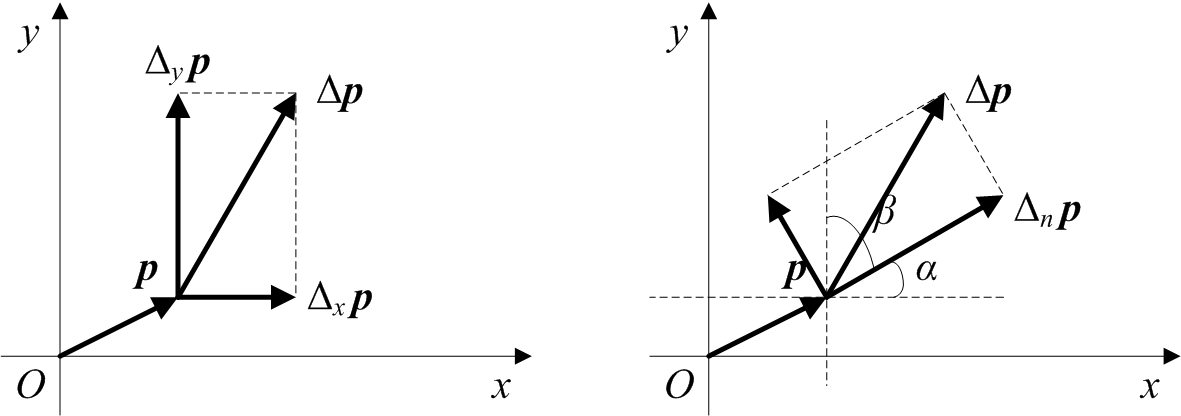
\includegraphics[height=3.5cm]{7.1.png}
\end{figure}

$\Delta _n\boldsymbol{p}$的表达式可以用坐标变换求得。
已知{\it xy}坐标系下的标准基及其构成的矩阵表示$A$:
\[
\boldsymbol{e}_1=\left( \begin{array}{c}
	1\\
	0\\
\end{array} \right) ,\boldsymbol{e}_2=\left( \begin{array}{c}
	0\\
	1\\
\end{array} \right) ,A=\left[ \begin{matrix}
	1&		0\\
	0&		1\\
\end{matrix} \right]
\]
新坐标系为原{\it xy}坐标系逆时针转$\alpha $,可得基及其构成的矩阵表示$W$:
\begin{align*}
&\because \begin{cases}
	L\left( \boldsymbol{e}_1 \right) =\left( \cos \alpha \,\,\sin \alpha \right) ^T\\
	L\left( \boldsymbol{e}_2 \right) =\left( -\sin \alpha \,\,\cos \alpha \right) ^T\\
\end{cases} \\
&\therefore W=\left[ \begin{matrix}
	\cos \alpha&		-\sin \alpha\\
	\sin \alpha&		\cos \alpha\\
\end{matrix} \right]
\end{align*}
由于:
\begin{align*}
&\because \Delta \boldsymbol{p}=A\left( \begin{array}{c}
	\Delta x\\
	\Delta y\\
\end{array} \right) =W\left( \begin{array}{c}
	\Delta n\\
	\Delta n_{\bot}\\
\end{array} \right) \\
&\therefore \left( \begin{array}{c}
	\Delta n\\
	\Delta n_{\bot}\\
\end{array} \right) =W^{-1}A\left( \begin{array}{c}
	\Delta x\\
	\Delta y\\
\end{array} \right) =\left( \begin{array}{c}
	\cos \alpha \Delta x+\sin \alpha \Delta y\\
	-\sin \alpha \Delta x+\cos \alpha \Delta y\\
\end{array} \right) \\
&\therefore \begin{cases}
	\Delta _n\boldsymbol{p}=\left( \begin{array}{c}
	\cos \alpha \Delta x+\sin \alpha \Delta y\\
	0\\
\end{array} \right)\\
	\Delta _{n_{\bot}}\boldsymbol{p}=\left( \begin{array}{c}
	0\\
	-\sin \alpha \Delta x+\cos \alpha \Delta y\\
\end{array} \right)\\
\end{cases}
\end{align*}
$\Delta _n\boldsymbol{p}$在{\it xy}坐标系下的表示:
\begin{align*}
&\because \Delta _n\boldsymbol{p}=A\left[ \Delta _n\boldsymbol{p} \right] _{xy}=W\left[ \Delta _n\boldsymbol{p} \right] _{nn_{\bot}}=W\left( \begin{array}{c}
	\cos \alpha \Delta x+\sin \alpha \Delta y\\
	0\\
\end{array} \right) \\
&\begin{aligned}
	\therefore \left[ \Delta _n\boldsymbol{p} \right] _{xy}&=\left[ \begin{matrix}
	\cos \alpha&		\sin \alpha\\
	-\sin \alpha&		\cos \alpha\\
\end{matrix} \right] \left( \begin{array}{c}
	\cos \alpha \Delta x+\sin \alpha \Delta y\\
	0\\
\end{array} \right)\\
    &=\left( \begin{array}{c}
	\cos \alpha \cos \alpha \Delta x+\sin \alpha \cos \alpha \Delta y\\
	-\sin \alpha \cos \alpha \Delta x-\sin \alpha \sin \alpha \Delta y\\
\end{array} \right)\\
	&=\left[ \begin{matrix}
	\cos \alpha \cos \alpha&		\sin \alpha \cos \alpha\\
	-\sin \alpha \cos \alpha&		-\sin \alpha \sin \alpha\\
\end{matrix} \right] \left( \begin{array}{c}
	\Delta x\\
	\Delta y\\
\end{array} \right)\\
	&=\left[ \begin{matrix}
	\cos \alpha \cos \alpha&		\cos \beta \cos \alpha\\
	-\cos \alpha \cos \beta&		-\cos \beta \cos \beta\\
\end{matrix} \right] \Delta \boldsymbol{p}\\
\end{aligned}
\end{align*}

\begin{tcolorbox}
这里需要重点弄清方向增量和全增量的关系。
\end{tcolorbox}

%============================================================
\subsection{因变量的增量}

\begin{definition}[因变量的增量]
若$z=f\left( \boldsymbol{p} \right) $,设开集$D$中的$\boldsymbol{p}$有偏增量$\Delta _x\boldsymbol{p},\Delta _y\boldsymbol{p}$,此时各自引起的$z$的增量称为{\bf 因变量$z$的偏增量},记为$\Delta _xz,\Delta _yz$,
同样地,若$\boldsymbol{p}$有全增量$\Delta \boldsymbol{p}$,则称引起的$z$的增量为{\bf 因变量$z$的全增量},记作$\Delta z$,
对应地,$\boldsymbol{p}$在$n$方向上的增量引起的$z$的增量称为{\bf 因变量$z$的方向增量},记作$\Delta _nz$,即:
\begin{align*}
&\Delta _xz=f\left( \boldsymbol{p}+\Delta _x\boldsymbol{p} \right) -f\left( \boldsymbol{p} \right) \\
&\Delta _yz=f\left( \boldsymbol{p}+\Delta _y\boldsymbol{p} \right) -f\left( \boldsymbol{p} \right) \\
&\Delta z=f\left( \boldsymbol{p}+\Delta \boldsymbol{p} \right) -f\left( \boldsymbol{p} \right) \\
&\Delta _nz=f\left( \boldsymbol{p}+\Delta _n\boldsymbol{p} \right) -f\left( \boldsymbol{p} \right)
\end{align*}
\end{definition}




